%% LaTeX2e class for student theses
%% sections/apendix.tex
%% 
%% Karlsruhe Institute of Technology
%% Institute for Program Structures and Data Organization
%% Chair for Software Design and Quality (SDQ)
%%
%% Dr.-Ing. Erik Burger
%% burger@kit.edu
%%
%% Version 1.1, 2014-11-21


%\iflanguage{english}
%{\chapter{Appendix}}    % english style
%{\chapter{Anhang}}      % german style
\chapter{Anhang}
\label{chap:appendix}


%\section{Fallbeispiel: Travelplanner}
%\label{sec:appendix:travelplanner}
		
\setcounter{figure}{0}

\begin{figure}[htp]
	\centering
  	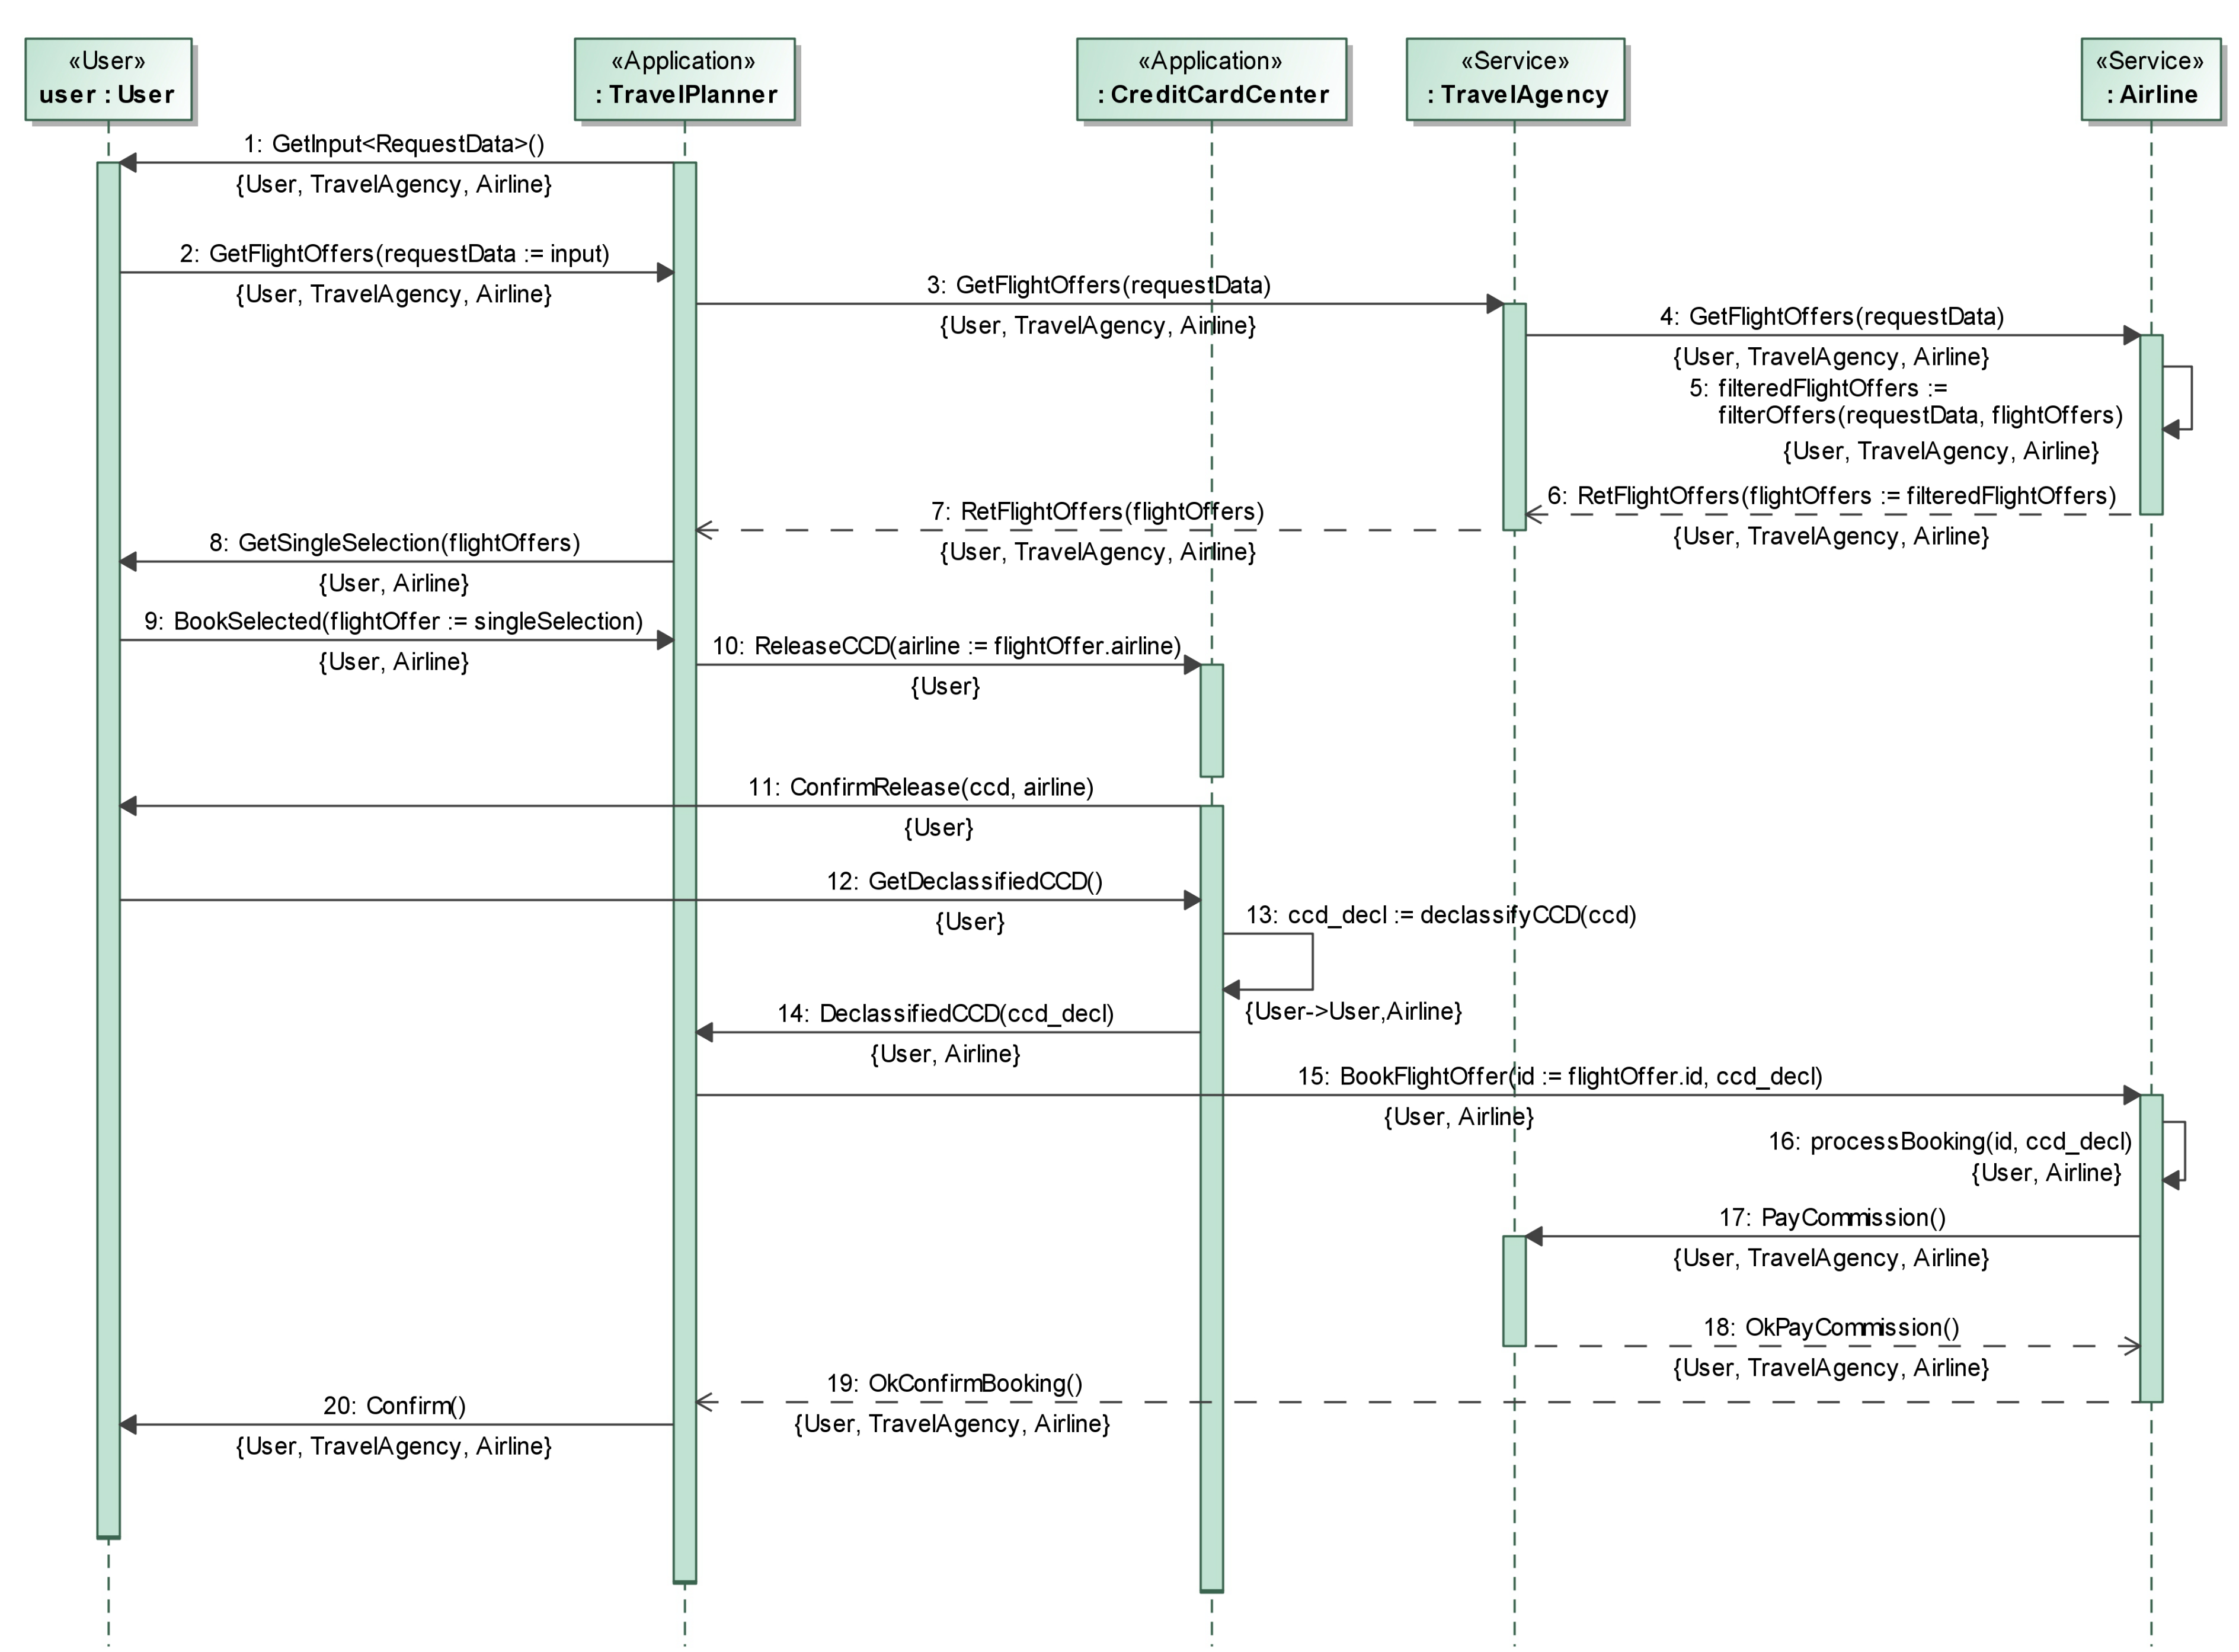
\includegraphics[width=1\textwidth]{images/travelplanner_seq_old.png}
	\caption{Sequenzdiagramm zur Buchung eines Fluges nach \cite{Stenzel2014}.}
	\label{sec:appendix:travelplanner:seq:old}
\end{figure}
	
\begin{figure}[htp]
	\centering
  	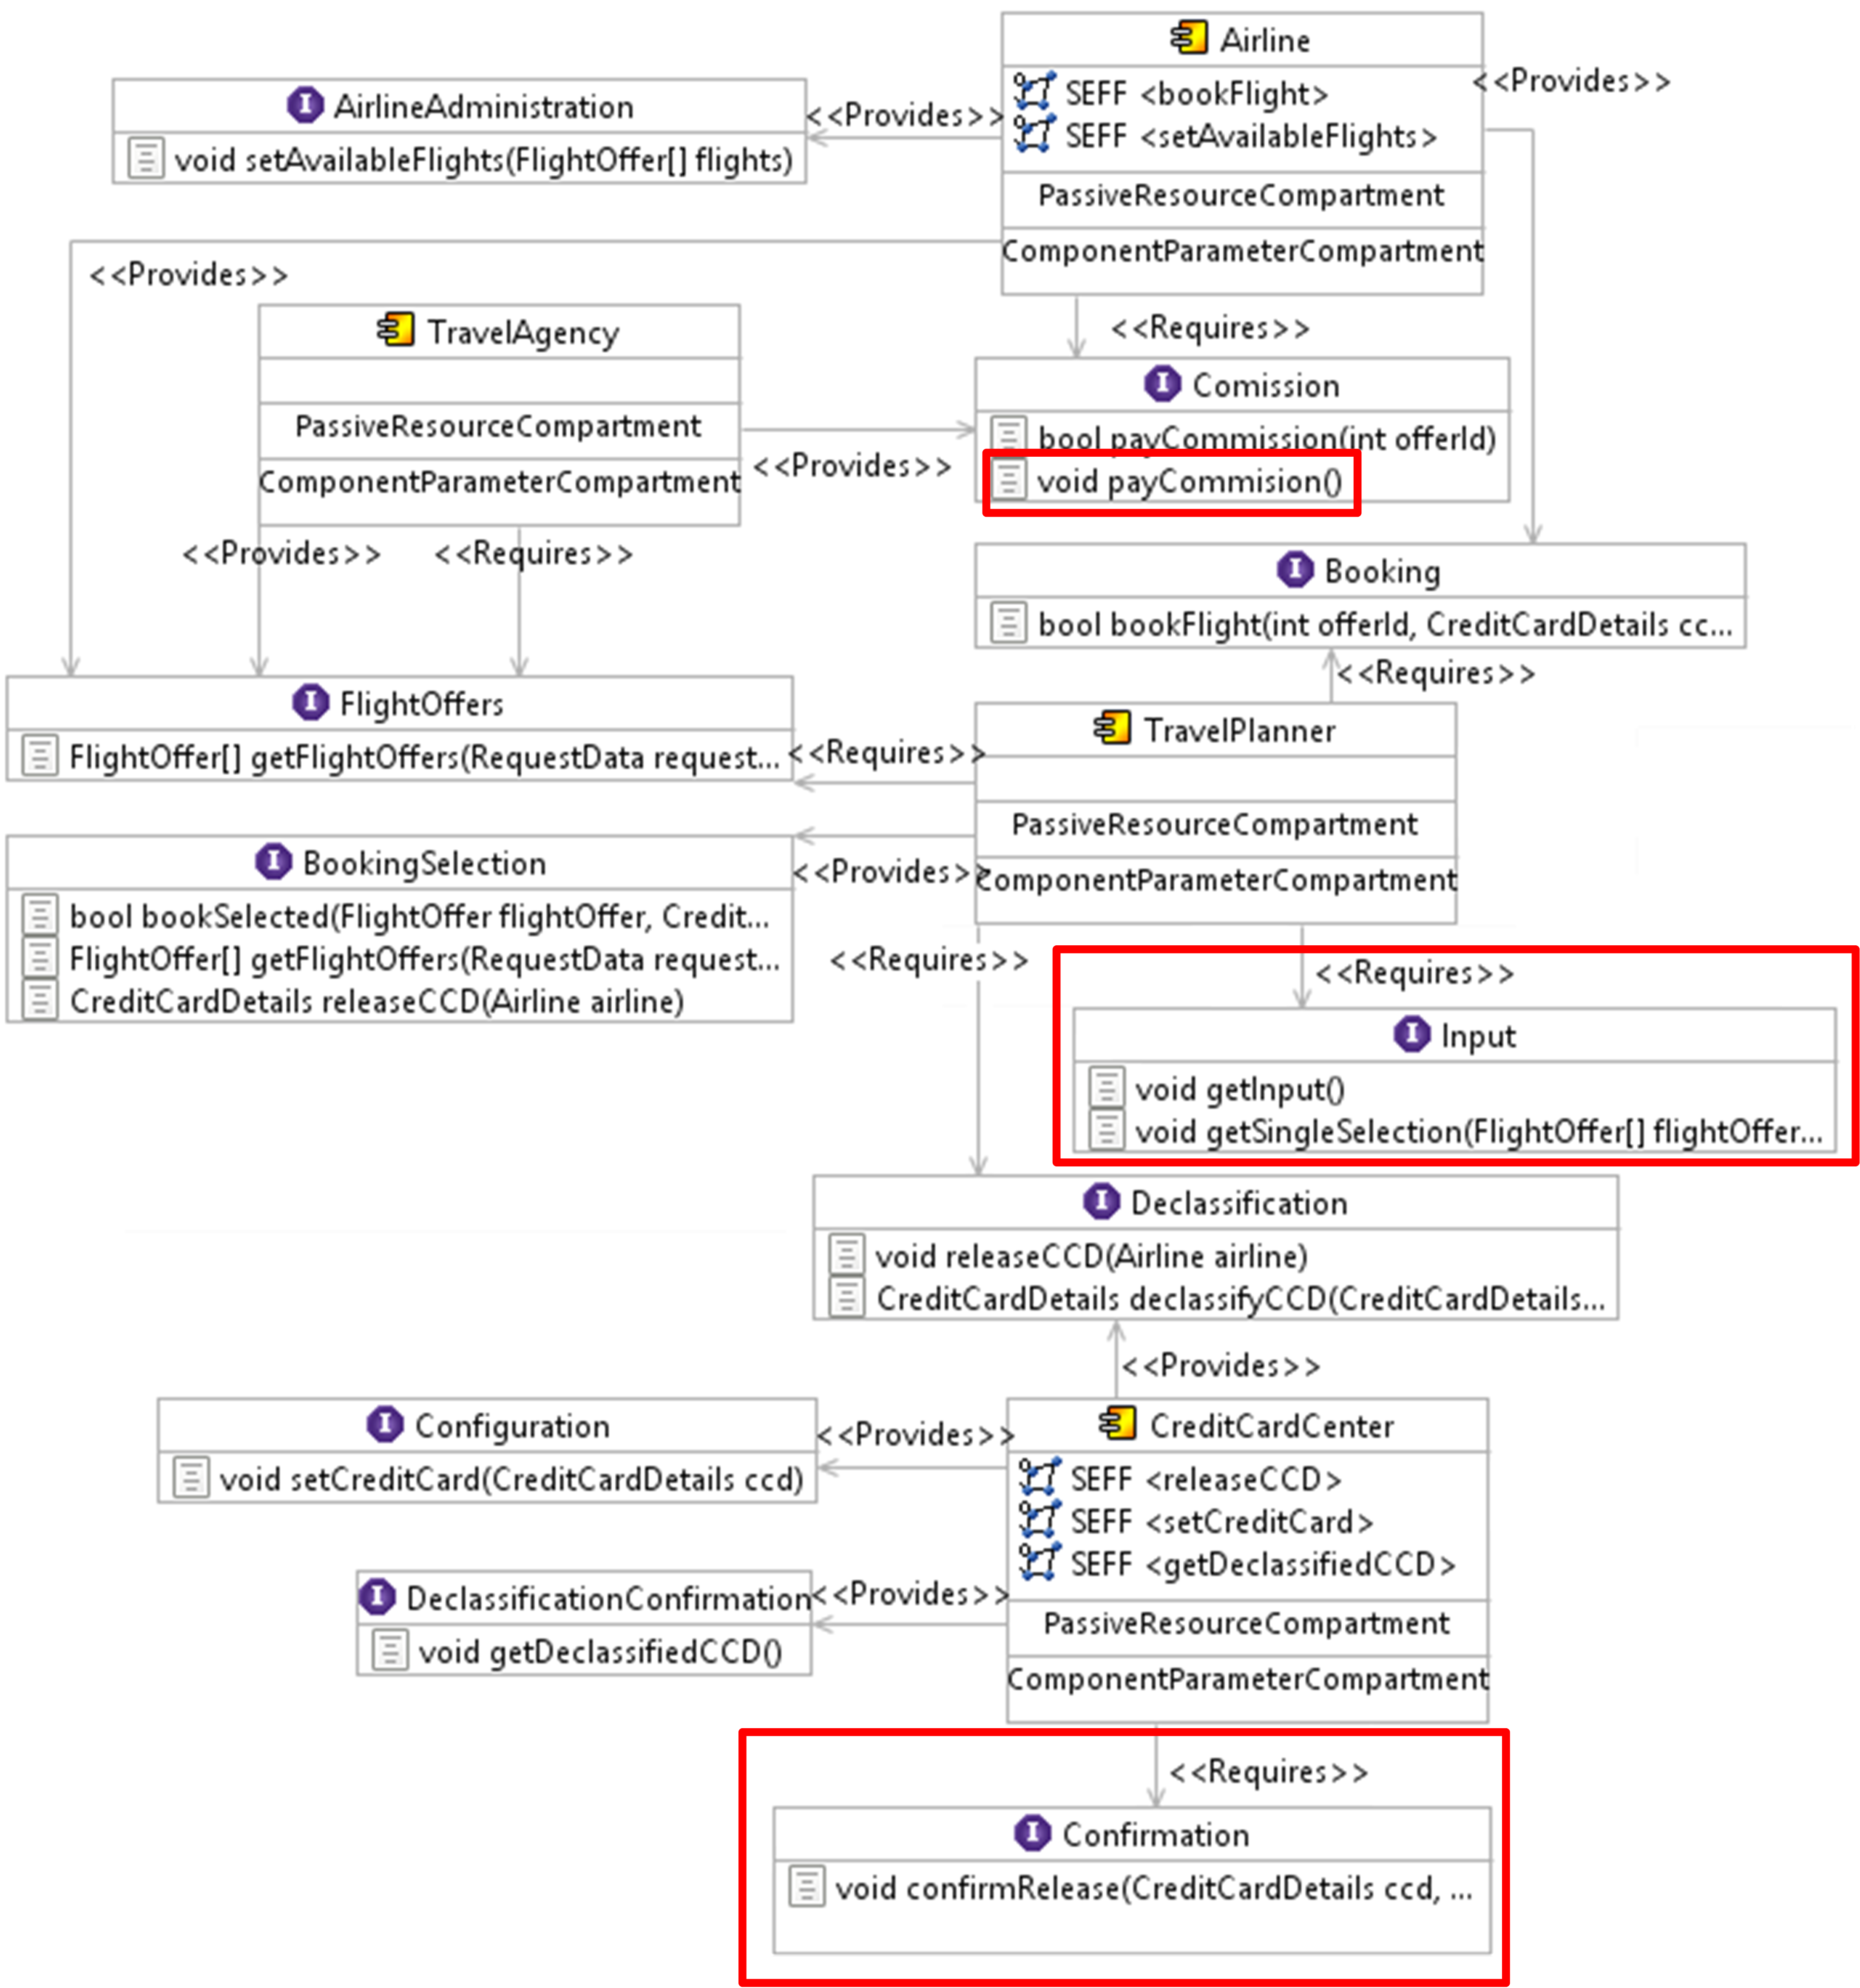
\includegraphics[height=0.7\textheight]{images/travelplanner_repository_edit.png}
	\caption{Komponenten-Repositoy-Modell des Travelplanner nach \cite{Kramera}. Markierte Elemente wurden entfernt}
	\label{sec:appendix:travelplanner:old:repo}
\end{figure}

\begin{figure}[htp]
	\centering
  	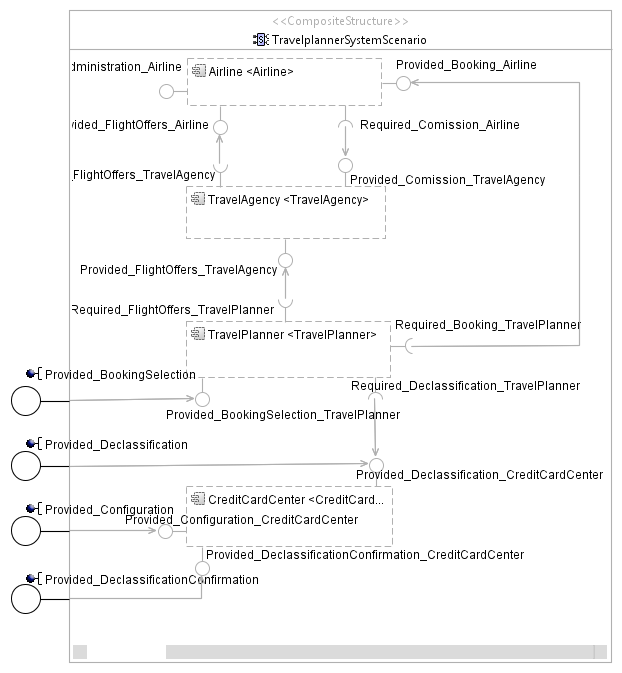
\includegraphics[height=0.7\textheight]{images/travelplanner_system.png}
	\caption{Systemmodell des Travelplanner}
	\label{sec:appendix:travelplanner:system}
\end{figure}

\begin{figure}[htp]
	\centering
  	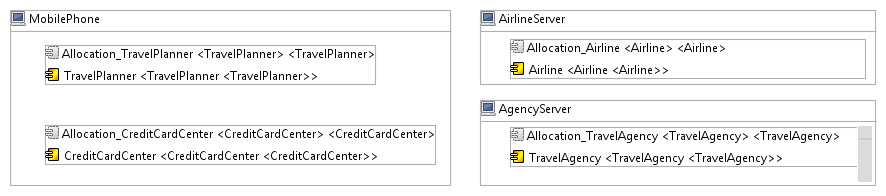
\includegraphics[width=1\textwidth]{images/travelplanner_allocation.png}
	\caption{Komponenten-Allokations-Modell des Travelplanner}
	\label{sec:appendix:travelplanner:allocation}
\end{figure}

%\section{Dokumentation Modellierung}
%\label{appendix:modell:doc}
